\documentclass{article}

\usepackage{fancyhdr}
\usepackage{extramarks}
\usepackage{amsmath}
\usepackage{amsthm}
\usepackage{amsfonts}
\usepackage{tikz}
\usepackage{graphicx} %插入图片的宏包
\usepackage{float} %设置图片浮动位置的宏包
\usepackage{pythonhighlight}
% \usepackage{subfigure} %插入多图时用子图显示的宏包
% \usepackage[plain]{algorithm}
% \usepackage{algpseudocode}

% \usetikzlibrary{automata,positioning}

%
% Basic Document Settings
%

\topmargin=-0.45in
\evensidemargin=0in
\oddsidemargin=0in
\textwidth=6.5in
\textheight=9.0in
\headsep=0.25in

\linespread{1.1}

\pagestyle{fancy}
\lhead{\hmwkAuthorName}
\chead{\hmwkClass\ : \hmwkTitle}
\rhead{\firstxmark}
\lfoot{\lastxmark}
\cfoot{\thepage}

\renewcommand\headrulewidth{0.4pt}
\renewcommand\footrulewidth{0.4pt}

\setlength\parindent{0pt}


%代码格式设置



%
% Create Problem Sections
%

\newcommand{\enterProblemHeader}[1]{
    \nobreak\extramarks{}{Problem \arabic{#1} continued on next page\ldots}\nobreak{}
    \nobreak\extramarks{Problem \arabic{#1} (continued)}{Problem \arabic{#1} continued on next page\ldots}\nobreak{}
}

\newcommand{\exitProblemHeader}[1]{
    \nobreak\extramarks{Problem \arabic{#1} (continued)}{Problem \arabic{#1} continued on next page\ldots}\nobreak{}
    \stepcounter{#1}
    \nobreak\extramarks{Problem \arabic{#1}}{}\nobreak{}
}

\setcounter{secnumdepth}{0}
\newcounter{partCounter}
\newcounter{homeworkProblemCounter}
\setcounter{homeworkProblemCounter}{1}
\nobreak\extramarks{Problem \arabic{homeworkProblemCounter}}{}\nobreak{}

%
% Homework Problem Environment
%
% This environment takes an optional argument. When given, it will adjust the
% problem counter. This is useful for when the problems given for your
% assignment aren't sequential. See the last 3 problems of this template for an
% example.
%
\newenvironment{homeworkProblem}[1][-1]{
    \ifnum#1>0
        \setcounter{homeworkProblemCounter}{#1}
    \fi
    \section{Problem \arabic{homeworkProblemCounter}}
    \setcounter{partCounter}{1}
    \enterProblemHeader{homeworkProblemCounter}
}{
    \exitProblemHeader{homeworkProblemCounter}
}

%
% Homework Details
%   - Title
%   - Due date
%   - Class
%   - Section/Time
%   - Instructor
%   - Author
%

\newcommand{\hmwkTitle}{Quiz\ \#6}
\newcommand{\hmwkDueDate}{Dec 23, 2018}
\newcommand{\hmwkClass}{Complex Networks}
\newcommand{\hmwkClassTime}{Section A}
% \newcommand{\hmwkClassInstructor}{Professor Isaac Newton}
\newcommand{\hmwkAuthorName}{\textbf{RUOPENG XU} }
\newcommand{\hmwkAuthorNum}{\textbf{18M38179} }

%
% Title Page
%

\title{
    \vspace{2in}
    \textmd{\textbf{\hmwkClass:\ \hmwkTitle}}\\
    \normalsize\vspace{0.1in}\small{Due\ on\ \hmwkDueDate\ }\\
    % \vspace{0.1in}\large{\textit{\hmwkClassInstructor\ \hmwkClassTime}}
    \vspace{3in}
}

\author{\hmwkAuthorName\\ \hmwkAuthorNum}
\date{}

\renewcommand{\part}[1]{\textbf{\large Part \Alph{partCounter}}\stepcounter{partCounter}\\}

%
% Various Helper Commands
%

% Useful for algorithms
\newcommand{\alg}[1]{\textsc{\bfseries \footnotesize #1}}

% For derivatives
\newcommand{\deriv}[1]{\frac{\mathrm{d}}{\mathrm{d}x} (#1)}

% For partial derivatives
\newcommand{\pderiv}[2]{\frac{\partial}{\partial #1} (#2)}

% Integral dx
\newcommand{\dx}{\mathrm{d}x}

% Alias for the Solution section header
\newcommand{\solution}{\textbf{\large Solution}}

% Probability commands: Expectation, Variance, Covariance, Bias
\newcommand{\E}{\mathrm{E}}
\newcommand{\Var}{\mathrm{Var}}
\newcommand{\Cov}{\mathrm{Cov}}
\newcommand{\Bias}{\mathrm{Bias}}

\begin{document}

\maketitle

\pagebreak

\begin{homeworkProblem}
    % questions
Make a program of computing (i) transitivity and (ii)
mean local clustering coefficient of (a) star graph, (b)
Petersen graph, (c) circle graph, (d) complete graph,
(e) complete bipartite graph, and (f) wheel graph.

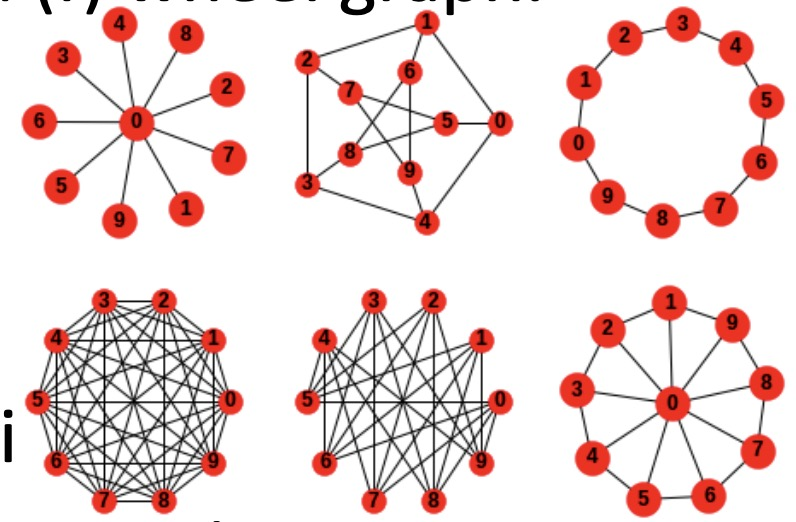
\includegraphics[scale=0.3]{quiz6_1.jpg}

\subsection*{Answer 1}

Use the bulid in function to compute the transitivity and mean local clustering coefficient:

\begin{python}
import networkx as nx
import matplotlib.pyplot as plt

star = nx.star_graph(9)
plt.subplot(231)
nx.draw(star, node_size=400, node_color='red', with_labels=True, font_weight='bold')
print("Transitivity of star:",nx.transitivity(star))
print("mean local clustering coefficient of star:",nx.average_clustering(star))


petersen = nx.petersen_graph()
plt.subplot(232)
nx.draw_shell(petersen, nlist=[range(5, 10), range(5)], node_size=200, node_color='red', with_labels=True, font_weight='bold')
print("Transitivity of petersen:",nx.transitivity(petersen))
print("mean local clustering coefficient of petersen:",nx.average_clustering(petersen))


cycle = nx.cycle_graph(10)
plt.subplot(233)
nx.draw_spring(cycle, node_size=400, node_color='red', with_labels=True, font_weight='bold')
print("Transitivity of cycle:",nx.transitivity(cycle))
print("mean local clustering coefficient of cycle:",nx.average_clustering(cycle))



K_10 = nx.complete_graph(10)
plt.subplot(234)
nx.draw_circular(K_10, node_size=200, node_color='red', with_labels=True, font_weight='bold')
print("Transitivity of K_10:",nx.transitivity(K_10))
print("mean local clustering coefficient of K_10:",nx.average_clustering(K_10))


K_5_5 = nx.complete_bipartite_graph(5, 5)
plt.subplot(235)
nx.draw_circular(K_5_5, nlist=[range(5, 10), range(5)], node_size=200, node_color='red', with_labels=True, font_weight='bold')
print("Transitivity of K_5_5:",nx.transitivity(K_5_5))
print("mean local clustering coefficient of K_5_5:",nx.average_clustering(K_5_5))



wheel = nx.wheel_graph(10)
plt.subplot(236)
nx.draw(wheel, node_size=400, node_color='red', with_labels=True, font_weight='bold')
print("Transitivity of wheel:",nx.transitivity(wheel))
print("mean local clustering coefficient of wheel:",nx.average_clustering(wheel))

\end{python}


The resule is as follows:

\begin{python}
Transitivity of star: 0
mean local clustering coefficient of star: 0.0

Transitivity of petersen: 0
mean local clustering coefficient of petersen: 0.0

Transitivity of cycle: 0
mean local clustering coefficient of cycle: 0.0

Transitivity of K_10: 1.0
mean local clustering coefficient of K_10: 1.0

Transitivity of K_5_5: 0
mean local clustering coefficient of K_5_5: 0.0

Transitivity of wheel: 0.42857142857142855
mean local clustering coefficient of wheel: 0.6250000000000001
\end{python}



\end{homeworkProblem}
\pagebreak


\end{document}
%
% Non sequential homework problems
%

% Jump to problem 18
